%%%%%%%%%%%%%%%%%%%%%%%%%%%%%%%%%%%%%%%%%%%%%%%%%%%%%%%%%%%%%%%%%%%%%%%%%%%%%%%%
\documentclass[twocolumn]{revtex4}

%%%%%%%%%%%%%%%%%%%%%%%%%%%%%%%%%%%%%%%%%%%%%%%%%%%%%%%%%%%%%%%%%%%%%%%%%%%%%%%%
% Note that comments begin with a "%" and are not turned into text in the .pdf
% document.
%%%%%%%%%%%%%%%%%%%%%%%%%%%%%%%%%%%%%%%%%%%%%%%%%%%%%%%%%%%%%%%%%%%%%%%%%%%%%%%%

%%%%%%%%%%%%%%%%%%%%%%%%%%%%%%%%%%%%%%%%%%%%%%%%%%%%%%%%%%%%%%%%%%%%%%%%%%%%%%%%
% Include some extra packages.
%%%%%%%%%%%%%%%%%%%%%%%%%%%%%%%%%%%%%%%%%%%%%%%%%%%%%%%%%%%%%%%%%%%%%%%%%%%%%%%%
\usepackage[]{graphicx}
%%%%%%%%%%%%%%%%%%%%%%%%%%%%%%%%%%%%%%%%%%%%%%%%%%%%%%%%%%%%%%%%%%%%%%%%%%%%%%%%

%%%%%%%%%%%%%%%%%%%%%%%%%%%%%%%%%%%%%%%%%%%%%%%%%%%%%%%%%%%%%%%%%%%%%%%%%%%%%%%%
\begin{document}

%%%%%%%%%%%%%%%%%%%%%%%%%%%%%%%%%%%%%%%%%%%%%%%%%%%%%%%%%%%%%%%%%%%%%%%%%%%%%%%%
\title{
Do you think it's possible to escape from a Raptor?  
}

\author{Isaiah Cameron-Murray}
\affiliation{Siena College, 515 Loudonville, NY}

\date{\today}

\begin{abstract}
    The project that we had to do was to figure out whether or not a raptor will catch me or if I could outrun it when given a 30 meter head start. I figured this out by using my knowledge on python. The speed of a human, which was 3m/s and the speed of a raptor, which was 18m/s. Both of these speeds were given to us by our professor. Using these numbers and my knowledge of physics I had to algebraically solve for the distance traveled and time that elapsed before it was one meter behind me. The reason why I had to do that was because I had to use that as a check to see if it was near or exactly the same number as what my python code outputted to me. Once I was able to get these numbers I had to calculate the percentage of whether or not I would escape from the raptor. The raptor would start to bite when it's one meter away on the first bite there is a 20 percent chance of it biting you, if it misses it will try again. On the second attempt there is a 15 percent chance of it biting you, and if it misses it will try one more time. On the third attempt there is a 7 percent chance of it biting you, and if it misses it will stop trying and you will get away. By using my knowledge on python i managed figure out my percentage of not getting bitten, which was between 62-63 percent.
    
\end{abstract}

\maketitle
%%%%%%%%%%%%%%%%%%%%%%%%%%%%%%%%%%%%%%%%%%%%%%%%%%%%%%%%%%%%%%%%%%%%%%%%%%%%%%%%

%%%%%%%%%%%%%%%%%%%%%%%%%%%%%%%%%%%%%%%%%%%%%%%%%%%%%%%%%%%%%%%%%%%%%%%%%%%%%%%%
\section{Introduction}

In these next couple of sections you will see the process of how I solved the problem in each question. You will also see the graphs I made and the equations I used to help me solve each problem. One basic kinematic equation used to help solve some of the questions was $x_f = x_0 + v\Delta(t) + \frac{1}{2}a(t)^2$.
%%%%%%%%%%%%%%%%%%%%%%%%%%%%%%%%%%%%%%%%%%%%%%%%%%%%%%%%%%%%%%%%%%%%%%%%%%%%%%%%


%%%%%%%%%%%%%%%%%%%%%%%%%%%%%%%%%%%%%%%%%%%%%%%%%%%%%%%%%%%%%%%%%%%%%%%%%%%%%%%%
\section{Problem 1: Position vs. Time}

\subsection{The Problem}
In this problem I was given the Raptors(18m/s) speed and also my own speed(3m/s). Also in the problem I was told that i had a 30 meter head start. The task that I was given in this problem was to properly label and plot a position vs. time graph for both me and the raptor.

\subsection{Python Code}
Before I did anything I had to import numpy as np and also import matplotlib.plylab as plt. What numpy does is it allows your python code to support complicated code like arrays and it also contains a library with math functions that allows the arrays to be used. Matplotlib is a plotting library and what it does is it allows me to graph whatever function I input into python. Then I wrote python code ''\%matplotlib inline'' and what this does is it allows the graph to show up inside the python code.
This next line 
$ x = np.linspace(0,10,10001)$
By using np.linspace it basically said to the program take 10001 points and evenly space them between 1 and 10. I didn't have to use 10001, I could have used any number but the more points you use the more accurate the graph becomes. To setup the next two equations I used $x_f = x_0 + v\Delta(t)$ as the base of my equation and then all I did was substitute the numbers that were given to me. In lines 8-15 were plotting functions that help form the graph. On line 8 and 9, the line that looks like this $plt.plot(x,y1,'y-',linewidth=2,label='Velociraptor speed')$. What this does is it plots the x and y values then next part connects the dots with a solid line and then it forms a legend. On lines 10 and 11 it labels the x and y axis. On lines 12 and 13 it sets the graph limit on the x and y axis. Line 14 gives a title to the graph and line 15 plots the graph. 

\subsection{Graph}
This is what the graph looks like.
\begin{figure}[h!]
\caption{Position vs. Time}
\centering
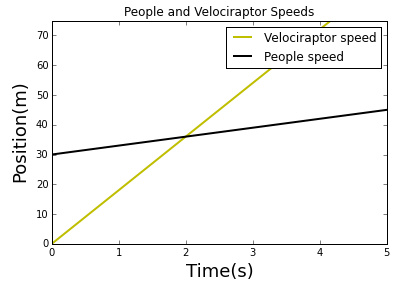
\includegraphics[width=.5\textwidth]{PvT_graph.png}
\end{figure}
%%%%%%%%%%%%%%%%%%%%%%%%%%%%%%%%%%%%%%%%%%%%


%%%%%%%%%%%%%%%%%%%%%%%%%%%%%%%%
\section{Problem 2: When does the 'raptor catch up to you?}

\subsection{The Problem}
In this problem I had to figure out when the raptor would catch up to me. As well as how long it took it to catch up to me.

\subsection{Python Code}
In this problem to figure out the distance and time I made a function called that took in the position of the Human(line2), the position of the raptor(line1), and the time values(t). The in that function i made a "for" loop that took a range of numbers between 0 and 10000. In that "for" loop I said "if" both the of the equations for the human and raptor are equal then return the time and position when both of the are equal to each other. The result that i got was it ran 36 meters and took 2 seconds to catch up to me.

\subsection{Calculations Used}
$$x_f = x_0 + v\Delta(t) + \frac{1}{2}a(t)^2$$
$$x_f =  v\Delta(t)$$
$$x_f = x_f$$
$$ x_0 + v_h\Delta(t)=  v_r\Delta(t)$$
$$\frac{x_0}{v_r - v_h} = t$$
$$ \frac{30m}{18- 3}=t$$
$$ t = 2s$$
$$x_f = v \Delta(t)$$
$$x_f = 18 \frac{m}{s}(2s)$$
$$x_f = 36m$$
The reason behind using no acceleration was in the beginning it was given that acceleration was not used which allowed me to manipulate the equation the way I did to get my answer. The function I made basically did all this for me.
%%%%%%%%%%%%%%%%%%%%%%%%%%%%%%%%%%%%%%%%%%%

%%%%%%%%%%%%%%%%%%%%%%%%%%%%%%%%%%%%
\section{Problem 3: When is it close enough to strike?}

\subsection{The Problem}
In this problem you find out that the raptor will start to attack when it is one meter behind you. The task was to find out how far you ran and how much time passed before the raptor was one meter behind. Then I had to graph it.

\subsection{Python Code}
For this question what i did in python to help me solve this was create a "for" loop. I said "for" i in range(len(y1)) and then in the loop i put an "if" statement. I said that if $y2[i]-y1[i]>1 and y2[i]-y1[i]<1.4$. This part of the if statement loops through and takes the time and looks for here the position of the person minus the position of the raptor is one.

The results I got was that the distance I ran before it was 1 meter away was 4.79 meters.The distance the raptor ran was 35.80 meters and the time that passed was 1.
Then after that in order to plot the graph I used the same method I used in problem 1.

\subsection{Graph}
T\begin{figure}[h!]
\caption{Position vs. Time}
\centering
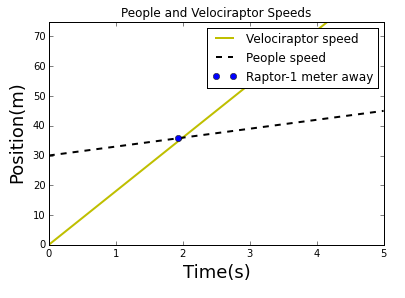
\includegraphics[width=.5\textwidth]{PvT_graph2.PNG}
\end{figure}his is the graph.

%%%%%%%%%%%%%%%%%%%%%%%%%%%%%%%%%%%%%%%%%%%
%%%%%%%%%%%%%%%%%%%%%%%%%%%%%%%%%%%%

%%%%%%%%%%%%%%%%%%%%%%%%%%%%%%%%%%%%%%%%%%

\section{Problem 4: Will it bite you?}

\subsection{The Problem}
For this problem I had to figure out the probability of me getting away. I was to that the first time it tries, there is a 20 percent chance it will get you. If it misses and it needs to try a second time, there is only a 15 percent chance, and if it misses that time, there is only a 7 percent chance on the third try.

\subsection{Python Code}
First what I did was made the variable $attempts = 10000$ then created a "for" loop that took the range of number between 0 and the number of attempts, which was 10000. With that in the loop I made another variable $ first = np.random.random()$ what this does is set the variable first equal to any random number. After I did that I made an "if" statement in the loop that basically said if those 10000 random numbers are greater than .2 which represents 20 percent then it would pass on to the next part of the loop. This would do the same thing for testing out and see if it was greater than 15 percent and 7 percent. Then I created another variable $probability = (float(prob)/attempts) * 100$ and what that did was take the  decimal number the python got and converted it to a percentage. The percentage that I got was between 62-63.8 percent.
%%%%%%%%%%%%%%%%%%%%%%%%%%%%%%%%%%%%%%%%%%
%%%%%%%%%%%%%%%%%%%%%%%%%%%%%%%%%%%%
\section{Conclusion}
Overall after doing all this coding the end results that I got was that when given a head start there is a high percentage in getting away. Even though that's crazy since it caught up in a matter of seconds. Maybe one of the reasons why the percentage is so big is because my dodging skill is so high. It took a while for me to rank that up ;) but needless to say there was a big probability of getting away.
%%%%%%%%%%%%%%%%%%%%%%%%%%%%%%%%%%%%%%%%%%
%%%%%%%%%%%%%%%%%%%%%%%%%%%%%%%%%%%%
\end{document}
%%%%%%%%%%%%%%%%%%%%%%%%%%%%%%%%%%%%%%%%%%%%%%%%%%%%%%%%%%%%%%%%%%%%%%%%%%%%%%%%

